\documentclass[
11pt, % The default document font size, options: 10pt, 11pt, 12pt
%codirector, % Uncomment to add a codirector to the title page
]{charter} 




% El títulos de la memoria, se usa en la carátula y se puede usar el cualquier lugar del documento con el comando \ttitle
\titulo{Sistema de gestión de lockers IoT} 

% Nombre del posgrado, se usa en la carátula y se puede usar el cualquier lugar del documento con el comando \degreename
\posgrado{Carrera de Especialización en Internet de las Cosas} 

% Tu nombre, se puede usar el cualquier lugar del documento con el comando \authorname
\autor{Lic. Leandro Percivati} 

% El nombre del director y co-director, se puede usar el cualquier lugar del documento con el comando \supname y \cosupname y \pertesupname y \pertecosupname
\director{Mg.Ing. Ericson Joseph Estupiñán Pineda}
\pertenenciaDirector{Surix} 
% FIXME:NO IMPLEMENTADO EL CODIRECTOR ni su pertenencia
%\codirector{No definido} % para que aparezca en la portada se debe descomentar la opción codirector en el documentclass
%\pertenenciaCoDirector{ }

% Nombre del cliente, quien va a aprobar los resultados del proyecto, se puede usar con el comando \clientename y \empclientename
\cliente{Ing. Sergio Starkloff}
\empresaCliente{Surix}

% Nombre y pertenencia de los jurados, se pueden usar el cualquier lugar del documento con el comando \jurunoname, \jurdosname y \jurtresname y \perteunoname, \pertedosname y \pertetresname.
%\juradoUno{No definido}
%\pertenenciaJurUno{ } 
%\juradoDos{No definido}
%\pertenenciaJurDos{ }
%\juradoTres{No definido}
%\pertenenciaJurTres{ }
 
\fechaINICIO{28 de febrero de 2023}		%Fecha de inicio de la cursada de GdP \fechaInicioName
\fechaFINALPlan{18 de abril de 2023} 	%Fecha de final de cursada de GdP
%\fechaFINALTrabajo{15 de mayo de 2022}	%Fecha de defensa pública del trabajo final


\begin{document}

\maketitle
\thispagestyle{empty}
\pagebreak


\thispagestyle{empty}
{\setlength{\parskip}{0pt}
\tableofcontents{}
}
\pagebreak


\section*{Registros de cambios}
\label{sec:registro}


\begin{table}[ht]
\label{tab:registro}
\centering
\begin{tabularx}{\linewidth}{@{}|c|X|c|@{}}
\hline
\rowcolor[HTML]{C0C0C0} 
Revisión & \multicolumn{1}{c|}{\cellcolor[HTML]{C0C0C0}Detalles de los cambios realizados} & Fecha      \\ \hline
0      & Creación del documento                                 & 28/02/2023 \\ \hline
1      & Se completa hasta el punto 5 inclusive                 & 13/03/2023 \\ \hline
2      & Se completa hasta el punto 9 inclusive 				& 21/03/2023 \\ \hline
%		  Se puede agregar algo más \newline
%		  En distintas líneas \newline
%		  Así                                                    & dd/mm/aaaa \\ \hline
%3      & Se completa hasta el punto 11 inclusive                & dd/mm/aaaa \\ \hline
%4      & Se completa el plan	                                 & dd/mm/aaaa \\ \hline
\end{tabularx}
\end{table}

\pagebreak



\section*{Acta de constitución del proyecto}
\label{sec:acta}

\begin{flushright}
Buenos Aires, \fechaInicioName
\end{flushright}

\vspace{2cm}

Por medio de la presente se acuerda con el \authorname\hspace{1px} que su Trabajo Final de la \degreename\hspace{1px} se titulará ``\ttitle'', consistirá esencialmente en la implementación de un prototipo de un sistema de control y manipulación de lockers, y tendrá un presupuesto preliminar estimado de 600 horas de trabajo, con fecha de inicio marzo de 2023 y fecha de presentación pública en diciembre de 2023.

Se adjunta a esta acta la planificación inicial.

\vfill

% Esta parte se construye sola con la información que hayan cargado en el preámbulo del documento y no debe modificarla
\begin{table}[ht]
\centering
\begin{tabular}{ccc}
\begin{tabular}[c]{@{}c@{}}Dr. Ing. Ariel Lutenberg \\ Director posgrado FIUBA\end{tabular} & \hspace{2cm} & \begin{tabular}[c]{@{}c@{}}\clientename \\ \empclientename \end{tabular} \vspace{2.5cm} \\ 
\multicolumn{3}{c}{\begin{tabular}[c]{@{}c@{}} \supname \\ Director del Trabajo Final\end{tabular}} \vspace{2.5cm} \\
%\begin{tabular}[c]{@{}c@{}}\jurunoname \\ Jurado del Trabajo Final\end{tabular}     &  & \begin{tabular}[c]{@{}c@{}}\jurdosname\\ Jurado del Trabajo Final\end{tabular}  \vspace{2.5cm}  \\
%\multicolumn{3}{c}{\begin{tabular}[c]{@{}c@{}} \jurtresname\\ Jurado del Trabajo Final\end{tabular}} \vspace{.5cm}                                                                     
\end{tabular}
\end{table}




\section{1. Descripción técnica-conceptual del proyecto a realizar}
\label{sec:descripcion}


Uno de los efectos inmediatos de la implementación de cuarentenas fue el gran crecimiento de compras online. Con el aumento de número de personas que comenzaron a trabajar desde su casa y la obligación de estar en el hogar durante la mayor parte del día, el modelo de compra online tuvo mucho éxito ya que evitaba que el comprador tenga contacto con otras personas y se contaba con que siempre habría alguien disponible para recibir los pedidos hechos.

Con la implementación de modelos híbridos de trabajo y la vuelta a la presencialidad de casi todas las actividades cotidianas, al modelo de compra online le surgió como desafío volver a asegurar la entrega de los pedidos ya que puede que no haya nadie para recibirlos.
Existen distintas formas de enfrentar este desafío. Muchas empresas ofrecen a través de su sistema, el seguimiento del pedido para que haya una persona en la casa al momento que este llegue. Sin embargo, los sistemas no contemplan imprevistos tanto del comprador (tener que salir del hogar aunque sepa que el pedido está en camino), como del repartidor (no poder cumplir con la entrega en el día pactado).

El objetivo de este proyecto es solucionar la problemática de requerir la presencia de una persona que reciba el pedido solicitado.
Para cumplir con el objetivo, el sistema debe ser informativo con el comprador (notificar estado del envío cada vez que haya un cambio) y seguro (evitar robos del pedido mientras no sea recibido por el comprador).

El caso de uso atendido por el sistema es el siguiente:

\begin{itemize}
	\item El repartidor llega a destino.
	\item Si el destinatario no se encuentra en el domicilio, el repartidor lo contacta por teléfono y le solicita el código de apertura del locker.
	\item El destinatario abre su aplicación móvil, solicita un código aleatorio al sistema y se lo informa al repartidor.
	\item Al recibirlo, el repartidor lo marca en el teclado del locker y este se abre, permitiendo que pueda guardar el pedido.
	\item El destinatario llega a su hogar y solicita un código aleatorio de apertura del locker a través de la aplicación.
	\item Al marcar el código en el teclado del locker, este se abre y el destinatario retira el pedido.
\end{itemize}

Adicionalmente, se contempla que existan tres tipos de servicios ofrecidos:
\begin{itemize}
	\item Lockers personales: solo un usuario puede hacer uso del mismo.
	\item Lockers compartidos: se considera esta opción por ejemplo para edificios, donde puede haber 6 lockers para 40 propietarios diferentes.
	\item Lockers en alquiler: pensado para negocios que quieran ofrecer el servicio de punto de entrega.
\end{itemize}

El sistema contará con aplicaciones (móvil y webapp), servidor y lockers, todos conectados por internet.
En la figura 1 se presenta el diagrama en bloques del sistema.

\begin{figure}[htpb]
\centering 
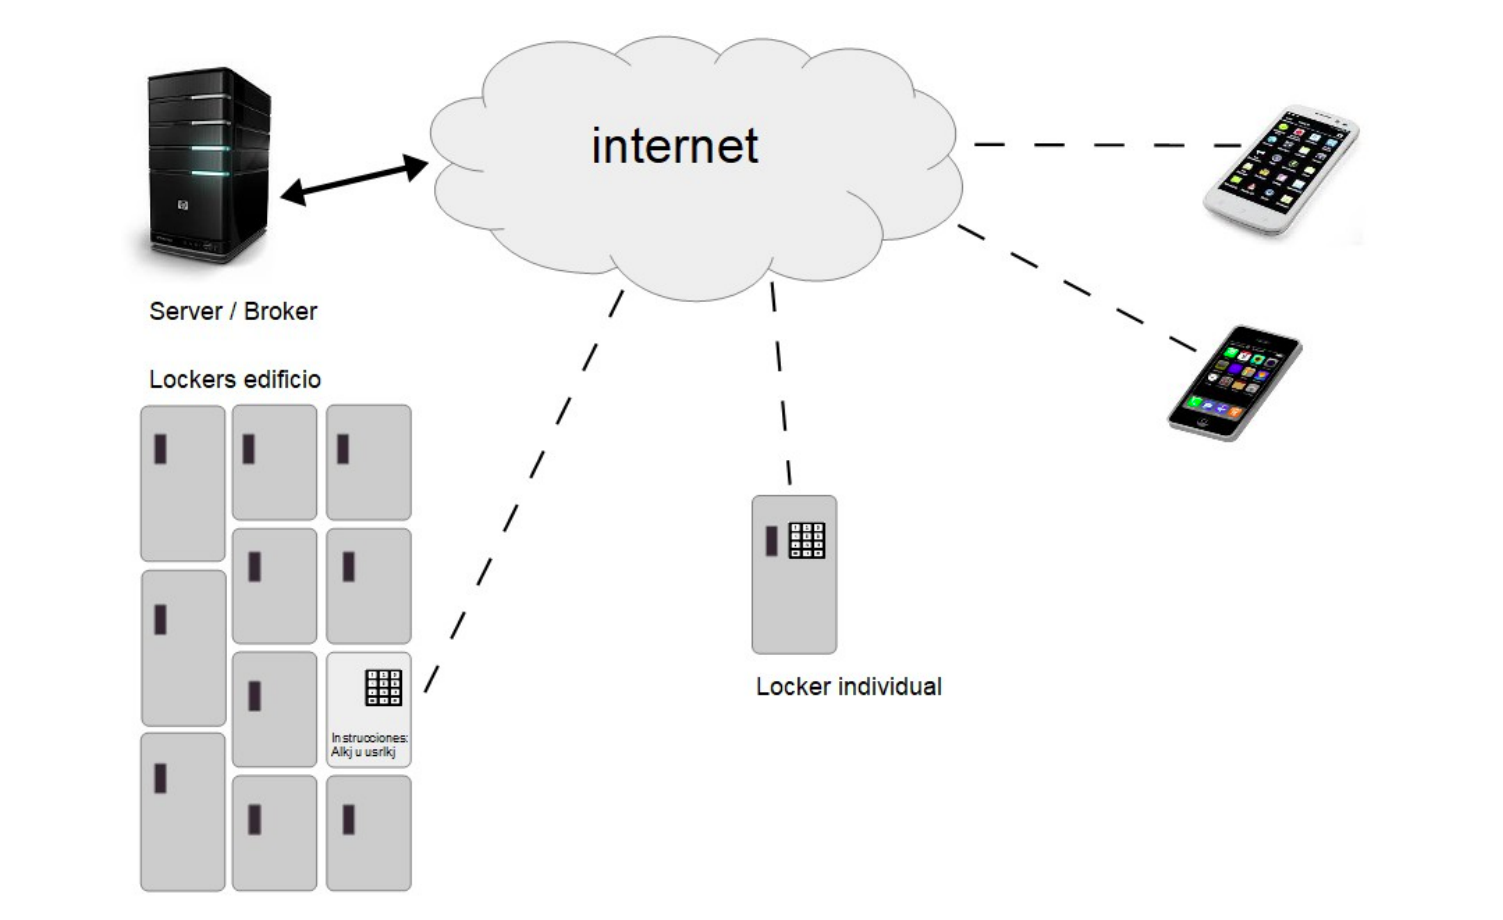
\includegraphics[width=1\textwidth]{./Figuras/diagrama.png}
\caption{Diagrama en bloques del sistema.}
\label{fig:diagBloques}
\end{figure}

\vspace{55px}

Por otra parte, se consideran tres roles en el sistema: usuarios, administradores y super administrador.
Los usuarios son quienes utilizan los lockers para guardar o retirar objetos.
En cuanto a los administradores, son aquellos que determinan qué usuarios pueden abrir los lockers. Esto permite que un mismo administrador otorgue permiso de uso de locker a diferentes usuarios en distintos momentos, como el caso de lockers compartidos o en alquiler. Además, pueden abrir los lockers.
El super administrador es un usuario especial, con derecho a gestionar sobre usuarios, administradores y lockers.

Por último, todas las acciones de los usuarios quedarán registradas para su consulta posterior. Esto se considera una parte importante del sistema ya que da el grado de seguridad que se tiene como objetivo.
Los registros permiten poder revisar el historial de un locker en caso del robo o pérdida de un pedido.



\section{2. Identificación y análisis de los interesados}
\label{sec:interesados}

\begin{table}[ht]
%\caption{Identificación de los interesados}
%\label{tab:interesados}
\begin{tabularx}{\linewidth}{@{}|l|X|X|l|@{}}
\hline
\rowcolor[HTML]{C0C0C0} 
Rol           & Nombre y Apellido & Organización 	& Puesto 	\\ \hline
%Auspiciante   &                   &              	&        	\\ \hline
Cliente       & \clientename      &\empclientename	& CTO      	\\ \hline
%Impulsor      &                   &              	&        	\\ \hline
Responsable   & \authorname       & FIUBA        	& Alumno 	\\ \hline
Colaboradores & Ericson Estupiñan & \empclientename & -       	\\ \hline
Orientador    & \supname	      & - 	& Director Trabajo final \\ \hline
%Orientador    & \supname	      & \pertesupname 	& Director Trabajo final \\ \hline
%Equipo        & miembro1 \newline 
%				miembro2          &              	&        	\\ \hline
%Opositores    &                   &              	&        	\\ \hline
Usuario final & Público general que quiera hacer uso de los lockers & - & - 	\\ \hline
\end{tabularx}
\end{table}

%El Director suele ser uno de los Orientadores.

%No dejar celdas vacías; si no hay nada que poner en una celda colocar un signo ``-''.

%No dejar filas vacías; si no hay nada que poner en una fila entonces eliminarla.

%Es deseable listar a continuación las principales características de cada interesado.
 
%Por ejemplo:
%\begin{itemize}
%	\item Auspiciante: es riguroso y exigente con la rendición de gastos. Tener mucho cuidado con esto.
%	\item Equipo: Juan Perez, suele pedir licencia porque tiene un familiar con una enfermedad. Planificar considerando esto.
%	\item Orientador: María Gómez va a poder ayudar mucho con la definición de los requerimientos.
%\end{itemize}



\section{3. Propósito del proyecto}
\label{sec:proposito}

El propósito de este proyecto es crear un sistema de gestión de lockers que estén conectados a internet, compuesto por un servidor broker, una web y una aplicación nativa para celulares.

\section{4. Alcance del proyecto}
\label{sec:alcance}

El proyecto incluye:

\begin{itemize}
	\item Estudio y desarrollo del protocolo MQTT, bases de datos, programación de aplicación web y multiplataforma.
	\item Desarrollo de servidor broker que orqueste la interacción con los lockers y usuarios.
	\item Desarrollo local de una página web que incluya alta de usuarios y acceso a datos guardados en base de datos.
    \item Desarrollo local de aplicación multiplataforma que permita solicitar códigos aleatorios a los usuarios, otorgar permiso de uso y reserva a los usuarios por parte de los administradores, alta de usuarios e inicio de sesión.
    \item Documentación del sistema desarrollado.
\end{itemize}

El proyecto no incluye:

\begin{itemize}
	\item Puesta en producción en el cliente final.
	\item Contratación de servicios cloud.
	\item Notificaciones en aplicación nativa.
    \item Traducciones a otros idiomas.
\end{itemize}


\section{5. Supuestos del proyecto}
\label{sec:supuestos}

Para el desarrollo del presente proyecto se supone que:

\begin{itemize}
	\item Se dispondrá de lockers con conectividad MQTT.
	\item Se dispondrá de computadora para instalación del servidor broker.
	\item Se dispondrá de bases de datos.
    \item La aplicación nativa se podrá montar sobre los sistemas operativos Android y iOS.
    \item Se contará con asistencia de colaboradores.
    \item Se dispondrá de 15 horas semanales dedicadas al proyecto.
    \item Se dispondrá de licencias de software en caso de que no se utilicen programas de código libre.	
\end{itemize}

\section{6. Requerimientos}
\label{sec:requerimientos}


\begin{enumerate}
	\item Requerimientos de la base de datos:
		\begin{enumerate}
			\item El sistema debe poseer una base de datos relacional.
			\item La base de datos debe contener las siguientes tablas:
				\begin{itemize}
					\item Usuarios.
					\item Lockers.
					\item Ubicaciones.
				    \item Roles.
					\item Permisos.
					\item Logs.
				\end{itemize}
			\item La base de datos debe tener datos cargados por default que permitan el correcto funcionamiento del sistema.
		\end{enumerate}
	\item Requerimientos del servidor backend:
		\begin{enumerate}
			\item Debe tener instalado un broker Eclipse Mosquitto con conectividad MQTT
			\item Debe interactuar con la base de datos para la consulta y guardado de información.
			\item Debe ofrecer endpoints con protocolo HTTP para interactuar tanto con la aplicación web como con la aplicación nativa.
		\end{enumerate}
	\item Requerimientos de la aplicación web:
		\begin{enumerate}
			\item Debe estar desarrollada en ReactJS.
			\item Debe soportar modelo de autenticación y autorización (login).
			\item Debe ofrecer la posibilidad de dar de alta, editar y ver usuarios del sistema.
			\item Debe ofrecer la posibilidad de dar de alta, editar y ver perfiles de usuarios.
			\item Debe ofrecer la posibilidad de dar de alta, editar y ver lockers del sistema.
			\item Debe ofrecer la posibilidad de ver las solicitudes de vinculación vigentes y asignarle uno o más lockers a cada usuario.
			\item Debe ofrecer la posibilidad de asignarle una ubicación a cada locker y/o a cada ubicación (existe posibilidad de una ubicación dentro de otra).
		\end{enumerate}
	\item Requerimientos de la aplicación nativa:
		\begin{enumerate}
			\item Debe estar desarrollada en React Native con framework Expo.
			\item Debe soportar modelo de autenticación y autorización (login).
			\item Debe ofrecer la posibilidad de escanear el código QR del locker solicitando la vinculación del usuario con el mismo.
			\item Debe ofrecer la posibilidad de solicitar un código aleatorio de apertura del locker vinculado.
			\item Debe ofrecer la posibilidad de abrir el locker vinculado.
		\end{enumerate}
	\item Requerimientos de la documentación:
		\begin{enumerate}
			\item Creación de documento con información detallada de la base de datos y de los servicios ofrecidos por la aplicación backend.
			\item Memoria del proyecto con diagramas UML de las aplicaciones y sus interacciones.
		\end{enumerate}		
	\item Requerimientos de pruebas:
		\begin{enumerate}
			\item Se realizarán pruebas integrales con los principales casos de uso requeridos.
		\end{enumerate}		
	\item Requerimientos de la entrega:
		\begin{enumerate}
			\item Se entregará el código en repositorio GitHub o GitLab en cuenta privada de la empresa.
		\end{enumerate}
\end{enumerate}


\section{7. Historias de usuarios (\textit{Product backlog})}
\label{sec:backlog}

Story points: se utilizará la serie de Fibonacci para estimar las historias de usuario. Cada puntaje corresponde a la suma estimada de dificultad de la historia junto al tamaño de desarrollo de la misma.

\begin{itemize}
	\item 1 Punto: Historias cortas y con dificultad baja.
	\item 2 Puntos: Historias con mayor tiempo de desarrollo y dificultad baja.
	\item 3 Puntos: Historias cortas pero con dificultad intermedia, pueden requerir investigar un tema en concreto o la conexión entre dos aplicaciones a través de una interfaz.
	\item 5 Puntos: Historias con mayor tiempo de desarrollo y dificultad intermedia.
	\item 8 Puntos: Historias con mucho tiempo de desarrollo pero dificultad baja o intermedia.
	\item 13 Puntos: Historias con mucho tiempo de desarrollo y con dificultad alta.
\end{itemize}

\begin{itemize}
	\item Como cliente quiero darme de alta en el sistema a través de la aplicación web: tiempo medio, dificultad media, 3 puntos.
	\item Como usuario quiero identificarme en la aplicación móvil: tiempo bajo, dificultad baja, 1 punto.
	\item Como usuario quiero identificarme en la aplicación web: tiempo bajo, dificultad baja, 1 punto.	
	\item Como usuario quiero ver los lockers vinculados en la aplicación móvil: tiempo medio, dificultad baja, 2 puntos.
	\item Como usuario quiero solicitar vinculación a un locker escaneando el código QR a través de la aplicación móvil: tiempo alto, dificultad media, 5 puntos.
	\item Como usuario quiero solicitar un código aleatorio de apertura de locker a través de la aplicación móvil: tiempo medio, dificultad media, 3 puntos.
	\item Como usuario quiero abrir locker a través de la aplicación móvil: tiempo alto, dificultad alta, 13 puntos.
	\item Como administrador quiero vincular un usuario a un locker a través de la aplicación web: tiempo medio, dificultad media, 3 puntos.
	\item Como super administrador quiero ver los perfiles del sistemas y sus permisos: tiempo medio, dificultad media, 3 puntos.
	\item Como super administrador quiero editar un perfil: tiempo medio, dificultad baja, 2 puntos.	
	\item Como super administrador quiero ver los lockers del sistema y sus ubicaciones: tiempo medio, dificultad media, 3 puntos.
	\item Como super administrador quiero dar de alta un nuevo locker a través de la aplicación web: tiempo medio, dificultad baja, 2 puntos.	
	\item Como super administrador quiero asignar un locker a una ubicación a través de la aplicación web: tiempo medio, dificultad baja, 2 puntos.	
\end{itemize}

\section{8. Entregables principales del proyecto}
\label{sec:entregables}

\begin{consigna}{red}

Los entregables del proyecto son (ejemplo):

\begin{itemize}
	\item Base de datos configurada con datos iniciales cargados
	\item Servidor con conectividad MQTT hacia los lockers y aplicación backend montada con conexión a la base de datos.
	\item Aplicación web desarrollada en React JS.
	\item Aplicación nativa desarrollada en React Native con framework Expo.
	\item Plan de proyecto y memoria técnica.
	\item Código del sistema en repositorio.
\end{itemize}

\end{consigna}

\section{9. Desglose del trabajo en tareas}
\label{sec:wbs}

\begin{enumerate}
\item Investigación inicial (70 hs):
	\begin{enumerate}
	\item Creación del plan de trabajo (10 hs).
	\item Investigación de tecnología NestJS para desarrollo del servidor backend (10 hs).
	\item Investigación de tecnología React JS para desarrollo de aplicación web (10 hs).
	\item Investigación de tecnología React Native para desarrollo de aplicación nativa (20 hs).
	\item Investigación del funcionamiento del broker Mosquitto y protocolo MQTT (20 hs).
	\end{enumerate}
\item Implementación de la base de datos (70 hs):
	\begin{enumerate}
	\item Diseño de la base de datos (20 hs).
	\item Creación de scripts de creación de tablas y cargado de información inicial (20 hs).
	\item Instalación de la base de datos (30 hs).
	\end{enumerate}
\item Implementación del servidor web (120 hs):
	\begin{enumerate}
	\item Instalación inicial y configuración del proyecto (10 hs).
	\item Instalación del broker MQTT y conexión con lockers (40 hs).
	\item Desarrollo de funciones para consulta y guardado de datos consumidos por las aplicaciones web y nativa (40 hs).
	\item Implementación de protocolos de seguridad y manejo de sesión (20 hs).
	\item Integración con servicio de mails para envío de mail de confirmación en creación de usuario (10 hs).
	\end{enumerate}
	
\item Implementación de la aplicación web (95 hs):
	\begin{enumerate}
	\item Creación del proyecto y estructura inicial (10 hs).
	\item Creación de página de alta de usuario (15 hs).
	\item Creación de página de autenticación de usuario (15 hs).
	\item Creación de página de administración de roles y perfiles(20 hs).	
	\item Creación de página de administración de usuarios (20 hs).
	\item Creación de página de administración de lockers y ubicaciones (15 hs).
	\end{enumerate}
	
\item Implementación de la aplicación nativa (130 hs):
	\begin{enumerate}
	\item Creación del proyecto y estructura inicial (25 hs).
	\item Creación de página de autenticación de usuario (20 hs).
	\item Creación de sección de escaneo QR y solicitud de vinculación con locker (35 hs).	
	\item Creación de página de visualización de lockers(15 hs).
	\item Creación de sección de locker con solicitud de código aleatorio, apertura y desvinculación (35 hs).
	\end{enumerate}	
	
\item Pruebas del sistema (55 hs):
	\begin{enumerate}
	\item Pruebas de aplicación web (10 hs).
	\item Pruebas de aplicación nativa (10 hs).
	\item Prueba integral con vinculación de usuario a locker y apertura desde la aplicación nativa (15 hs).	
	\item Prueba integral con vinculación de usuario a locker y generación de código aleatorio desde la aplicación nativa (10 hs).	
	\item Prueba integral con desvinculación de usuario a locker (10 hs).	
	\end{enumerate}	
	
\item Documentación técnica del proyecto (60 hs):
	\begin{enumerate}
	\item Creación de informe de avance (10 hs).
	\item Redacción de la memoria técnica del proyecto (50 hs).
	\end{enumerate}	
\end{enumerate}

Cantidad total de horas: (tantas h)

\section{10. Diagrama de Activity On Node}
\label{sec:AoN}

\begin{consigna}{red}
Armar el AoN a partir del WBS definido en la etapa anterior. 

%La figura \ref{fig:AoN} fue elaborada con el paquete latex tikz y pueden consultar la siguiente referencia \textit{online}:

%\url{https://www.overleaf.com/learn/latex/LaTeX_Graphics_using_TikZ:_A_Tutorial_for_Beginners_(Part_3)\%E2\%80\%94Creating_Flowcharts}

\end{consigna}

\begin{figure}[htpb]
\centering 
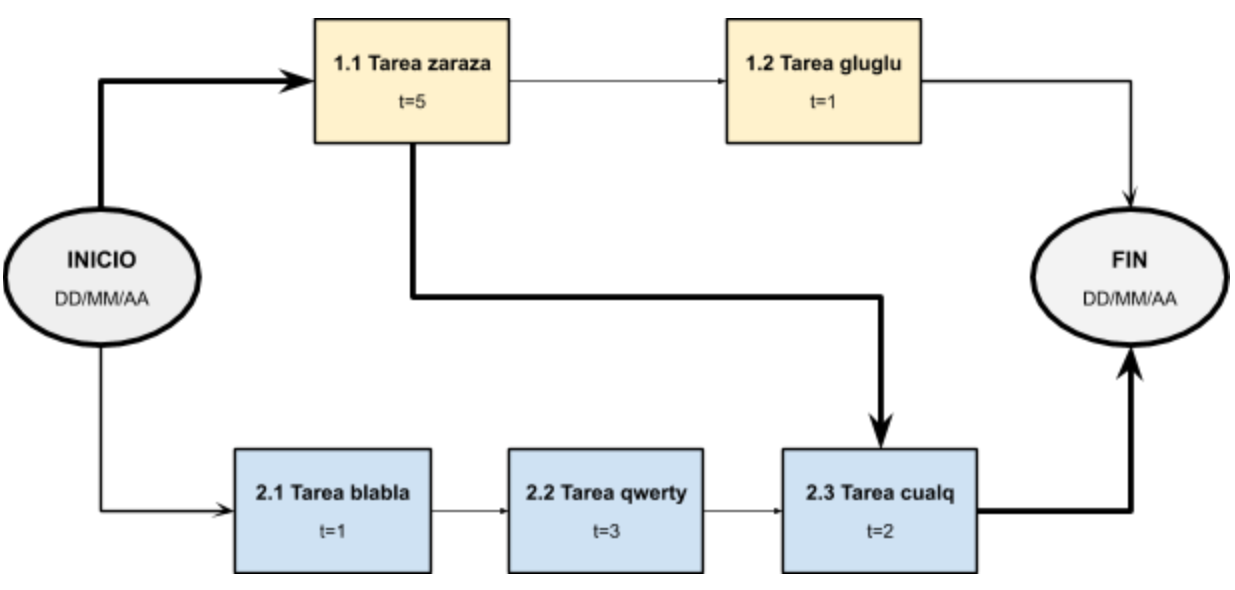
\includegraphics[width=.8\textwidth]{./Figuras/AoN.png}
\caption{Diagrama de \textit{Activity on Node}.}
\label{fig:AoN}
\end{figure}

Indicar claramente en qué unidades están expresados los tiempos.
De ser necesario indicar los caminos semicríticos y analizar sus tiempos mediante un cuadro.
Es recomendable usar colores y un cuadro indicativo describiendo qué representa cada color, como se muestra en el siguiente ejemplo:



\section{11. Diagrama de Gantt}
\label{sec:gantt}

\begin{consigna}{red}

Existen muchos programas y recursos \textit{online} para hacer diagramas de Gantt, entre los cuales destacamos:

\begin{itemize}
\item Planner
\item GanttProject
\item Trello + \textit{plugins}. En el siguiente link hay un tutorial oficial: \\ \url{https://blog.trello.com/es/diagrama-de-gantt-de-un-proyecto}
\item Creately, herramienta online colaborativa. \\\url{https://creately.com/diagram/example/ieb3p3ml/LaTeX}
\item Se puede hacer en latex con el paquete \textit{pgfgantt}\\ \url{http://ctan.dcc.uchile.cl/graphics/pgf/contrib/pgfgantt/pgfgantt.pdf}
\end{itemize}

Pegar acá una captura de pantalla del diagrama de Gantt, cuidando que la letra sea suficientemente grande como para ser legible. 
Si el diagrama queda demasiado ancho, se puede pegar primero la ``tabla'' del Gantt y luego pegar la parte del diagrama de barras del diagrama de Gantt.

Configurar el software para que en la parte de la tabla muestre los códigos del EDT (WBS).\\
Configurar el software para que al lado de cada barra muestre el nombre de cada tarea.\\
Revisar que la fecha de finalización coincida con lo indicado en el Acta Constitutiva.

En la figura \ref{fig:gantt}, se muestra un ejemplo de diagrama de Gantt realizado con el paquete de \textit{pgfgantt}. En la plantilla pueden ver el código que lo genera y usarlo de base para construir el propio.

\begin{figure}[htbp]
\begin{center}
\begin{ganttchart}{1}{12}
  \gantttitle{2020}{12} \\
  \gantttitlelist{1,...,12}{1} \\
  \ganttgroup{Group 1}{1}{7} \\
  \ganttbar{Task 1}{1}{2} \\
  \ganttlinkedbar{Task 2}{3}{7} \ganttnewline
  \ganttmilestone{Milestone o hito}{7} \ganttnewline
  \ganttbar{Final Task}{8}{12}
  \ganttlink{elem2}{elem3}
  \ganttlink{elem3}{elem4}
\end{ganttchart}
\end{center}
\caption{Diagrama de Gantt de ejemplo}
\label{fig:gantt}
\end{figure}


\begin{landscape}
\begin{figure}[htpb]
\centering 
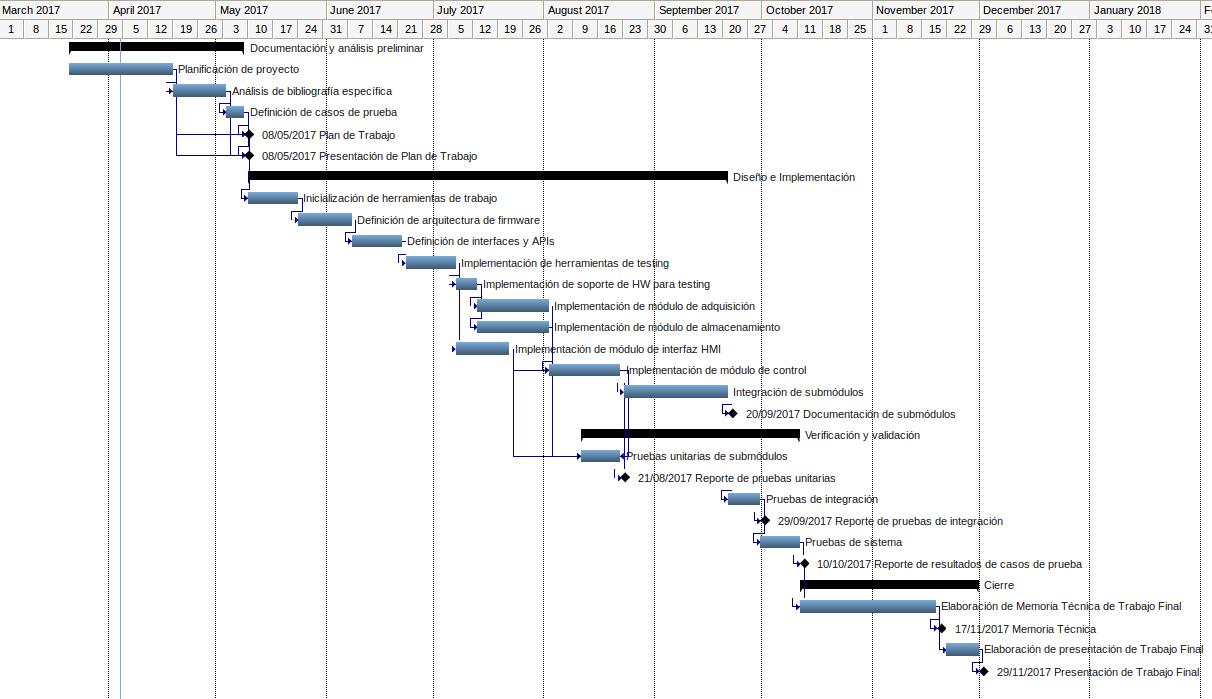
\includegraphics[height=.85\textheight]{./Figuras/Gantt-2.png}
\caption{Ejemplo de diagrama de Gantt rotado}
\label{fig:diagGantt}
\end{figure}

\end{landscape}

\end{consigna}


\section{12. Presupuesto detallado del proyecto}
\label{sec:presupuesto}

\begin{consigna}{red}
Si el proyecto es complejo entonces separarlo en partes:
\begin{itemize}
	\item Un total global, indicando el subtotal acumulado por cada una de las áreas.
	\item El desglose detallado del subtotal de cada una de las áreas.
\end{itemize}

IMPORTANTE: No olvidarse de considerar los COSTOS INDIRECTOS.

\end{consigna}

\begin{table}[htpb]
\centering
\begin{tabularx}{\linewidth}{@{}|X|c|r|r|@{}}
\hline
\rowcolor[HTML]{C0C0C0} 
\multicolumn{4}{|c|}{\cellcolor[HTML]{C0C0C0}COSTOS DIRECTOS} \\ \hline
\rowcolor[HTML]{C0C0C0} 
Descripción &
  \multicolumn{1}{c|}{\cellcolor[HTML]{C0C0C0}Cantidad} &
  \multicolumn{1}{c|}{\cellcolor[HTML]{C0C0C0}Valor unitario} &
  \multicolumn{1}{c|}{\cellcolor[HTML]{C0C0C0}Valor total} \\ \hline
 &
  \multicolumn{1}{c|}{} &
  \multicolumn{1}{c|}{} &
  \multicolumn{1}{c|}{} \\ \hline
 &
  \multicolumn{1}{c|}{} &
  \multicolumn{1}{c|}{} &
  \multicolumn{1}{c|}{} \\ \hline
\multicolumn{1}{|l|}{} &
   &
   &
   \\ \hline
\multicolumn{1}{|l|}{} &
   &
   &
   \\ \hline
\multicolumn{3}{|c|}{SUBTOTAL} &
  \multicolumn{1}{c|}{} \\ \hline
\rowcolor[HTML]{C0C0C0} 
\multicolumn{4}{|c|}{\cellcolor[HTML]{C0C0C0}COSTOS INDIRECTOS} \\ \hline
\rowcolor[HTML]{C0C0C0} 
Descripción &
  \multicolumn{1}{c|}{\cellcolor[HTML]{C0C0C0}Cantidad} &
  \multicolumn{1}{c|}{\cellcolor[HTML]{C0C0C0}Valor unitario} &
  \multicolumn{1}{c|}{\cellcolor[HTML]{C0C0C0}Valor total} \\ \hline
\multicolumn{1}{|l|}{} &
   &
   &
   \\ \hline
\multicolumn{1}{|l|}{} &
   &
   &
   \\ \hline
\multicolumn{1}{|l|}{} &
   &
   &
   \\ \hline
\multicolumn{3}{|c|}{SUBTOTAL} &
  \multicolumn{1}{c|}{} \\ \hline
\rowcolor[HTML]{C0C0C0}
\multicolumn{3}{|c|}{TOTAL} &
   \\ \hline
\end{tabularx}%
\end{table}


\section{13. Gestión de riesgos}
\label{sec:riesgos}

\begin{consigna}{red}
a) Identificación de los riesgos (al menos cinco) y estimación de sus consecuencias:
 
Riesgo 1: detallar el riesgo (riesgo es algo que si ocurre altera los planes previstos de forma negativa)
\begin{itemize}
	\item Severidad (S): mientras más severo, más alto es el número (usar números del 1 al 10).\\
	Justificar el motivo por el cual se asigna determinado número de severidad (S).
	\item Probabilidad de ocurrencia (O): mientras más probable, más alto es el número (usar del 1 al 10).\\
	Justificar el motivo por el cual se asigna determinado número de (O). 
\end{itemize}   

Riesgo 2:
\begin{itemize}
	\item Severidad (S): 
	\item Ocurrencia (O):
\end{itemize}

Riesgo 3:
\begin{itemize}
	\item Severidad (S): 
	\item Ocurrencia (O):
\end{itemize}


b) Tabla de gestión de riesgos:      (El RPN se calcula como RPN=SxO)

\begin{table}[htpb]
\centering
\begin{tabularx}{\linewidth}{@{}|X|c|c|c|c|c|c|@{}}
\hline
\rowcolor[HTML]{C0C0C0} 
Riesgo & S & O & RPN & S* & O* & RPN* \\ \hline
       &   &   &     &    &    &      \\ \hline
       &   &   &     &    &    &      \\ \hline
       &   &   &     &    &    &      \\ \hline
       &   &   &     &    &    &      \\ \hline
       &   &   &     &    &    &      \\ \hline
\end{tabularx}%
\end{table}

Criterio adoptado: 
Se tomarán medidas de mitigación en los riesgos cuyos números de RPN sean mayores a...

Nota: los valores marcados con (*) en la tabla corresponden luego de haber aplicado la mitigación.

c) Plan de mitigación de los riesgos que originalmente excedían el RPN máximo establecido:
 
Riesgo 1: plan de mitigación (si por el RPN fuera necesario elaborar un plan de mitigación).
  Nueva asignación de S y O, con su respectiva justificación:
  - Severidad (S): mientras más severo, más alto es el número (usar números del 1 al 10).
          Justificar el motivo por el cual se asigna determinado número de severidad (S).
  - Probabilidad de ocurrencia (O): mientras más probable, más alto es el número (usar del 1 al 10).
          Justificar el motivo por el cual se asigna determinado número de (O).

Riesgo 2: plan de mitigación (si por el RPN fuera necesario elaborar un plan de mitigación).
 
Riesgo 3: plan de mitigación (si por el RPN fuera necesario elaborar un plan de mitigación).

\end{consigna}


\section{14. Gestión de la calidad}
\label{sec:calidad}

\begin{consigna}{red}
Para cada uno de los requerimientos del proyecto indique:
\begin{itemize} 
\item Req \#1: copiar acá el requerimiento.

\begin{itemize}
	\item Verificación para confirmar si se cumplió con lo requerido antes de mostrar el sistema al cliente. Detallar 
	\item Validación con el cliente para confirmar que está de acuerdo en que se cumplió con lo requerido. Detallar  
\end{itemize}

\end{itemize}

Tener en cuenta que en este contexto se pueden mencionar simulaciones, cálculos, revisión de hojas de datos, consulta con expertos, mediciones, etc.  Las acciones de verificación suelen considerar al entregable como ``caja blanca'', es decir se conoce en profundidad su funcionamiento interno.  En cambio, las acciones de validación suelen considerar al entregable como ``caja negra'', es decir, que no se conocen los detalles de su funcionamiento interno.

\end{consigna}

\section{15. Procesos de cierre}    
\label{sec:cierre}

\begin{consigna}{red}
Establecer las pautas de trabajo para realizar una reunión final de evaluación del proyecto, tal que contemple las siguientes actividades:

\begin{itemize}
	\item Pautas de trabajo que se seguirán para analizar si se respetó el Plan de Proyecto original:
	 - Indicar quién se ocupará de hacer esto y cuál será el procedimiento a aplicar. 
	\item Identificación de las técnicas y procedimientos útiles e inútiles que se emplearon, y los problemas que surgieron y cómo se solucionaron:
	 - Indicar quién se ocupará de hacer esto y cuál será el procedimiento para dejar registro.
	\item Indicar quién organizará el acto de agradecimiento a todos los interesados, y en especial al equipo de trabajo y colaboradores:
	  - Indicar esto y quién financiará los gastos correspondientes.
\end{itemize}

\end{consigna}


\end{document}
